%Wie im Abschnitt zuvor erwähnt, wird in diesem Abschnitt die Extraktion des Signals, beziehungsweise die Abschätzung des korrelierten Untergrunds durch Parametrisieren von Funktionen kurz vorgestellt.
%\newline
Da es sich bei dem Signal um eine statistische Größe handelt, wird eine gaußförmig Funktion benutzt, um das Signal zu beschreiben.
%Der Mittelwert der Signalfunktion stellt einen freien Parameter dar und entspricht im Optimalfall der $\pi^{0}$-Masse.
%Als zwei weitere freie Parameter werden die Amplitude der Signalfunktion, sowie die Standardabweichung vom Mittelwert benutzt.
\newline
Wie bereits diskutiert, können Photonenkandidaten aus Konversionen eine geringere Energie tragen, als nicht konvertierte Photonenkandidaten.
Dadurch liegt die                                                                                                                                                                                                                                                                                                                                                                                                                                                                                                                                                                                                                                                                                                                                                                                                                                                                                                                                                                                                                                                                                                                                                                                                                                                                                                                                                                                                                                                                                                                                                                                                       e Masse in Kombinationen mit Photonenkandidaten aus Konversionen bei kleineren Werten, als die $\pi^{0}$ Masse, obwohl die Photonenkandidaten von dem gleichen $\pi^{0}$ stammen.
Deshalb wird die gaußförmig Funktion zur Beschreibung des Signals um eine sogenannte \textit{Tail} Komponente erweitert.
Die \textit{Tail} Komponente wird durch eine exponentielle Funktion beschrieben, die anschaulich als eine Abweichung der gaußförmig Funktion des Signals auf der linken Seite der $\pi^{0}$ Masse betrachtet werden kann.
\newline
Für den korrelierten Untergrund wird eine lineare Funktion, abhängig von der invarianten Masse, angenommen.
\newline
Die drei Funktionen werden zusammen durch Variation ihrer freien Parameter an die Verteilung angepasst.
Als freie Parameter für den korrelierten Untergrund wird der Schnittpunkt mit der y-Achse, sowie die Steigung der linearen Funktion verwendet.
\begin{figure}[tp]
\centering
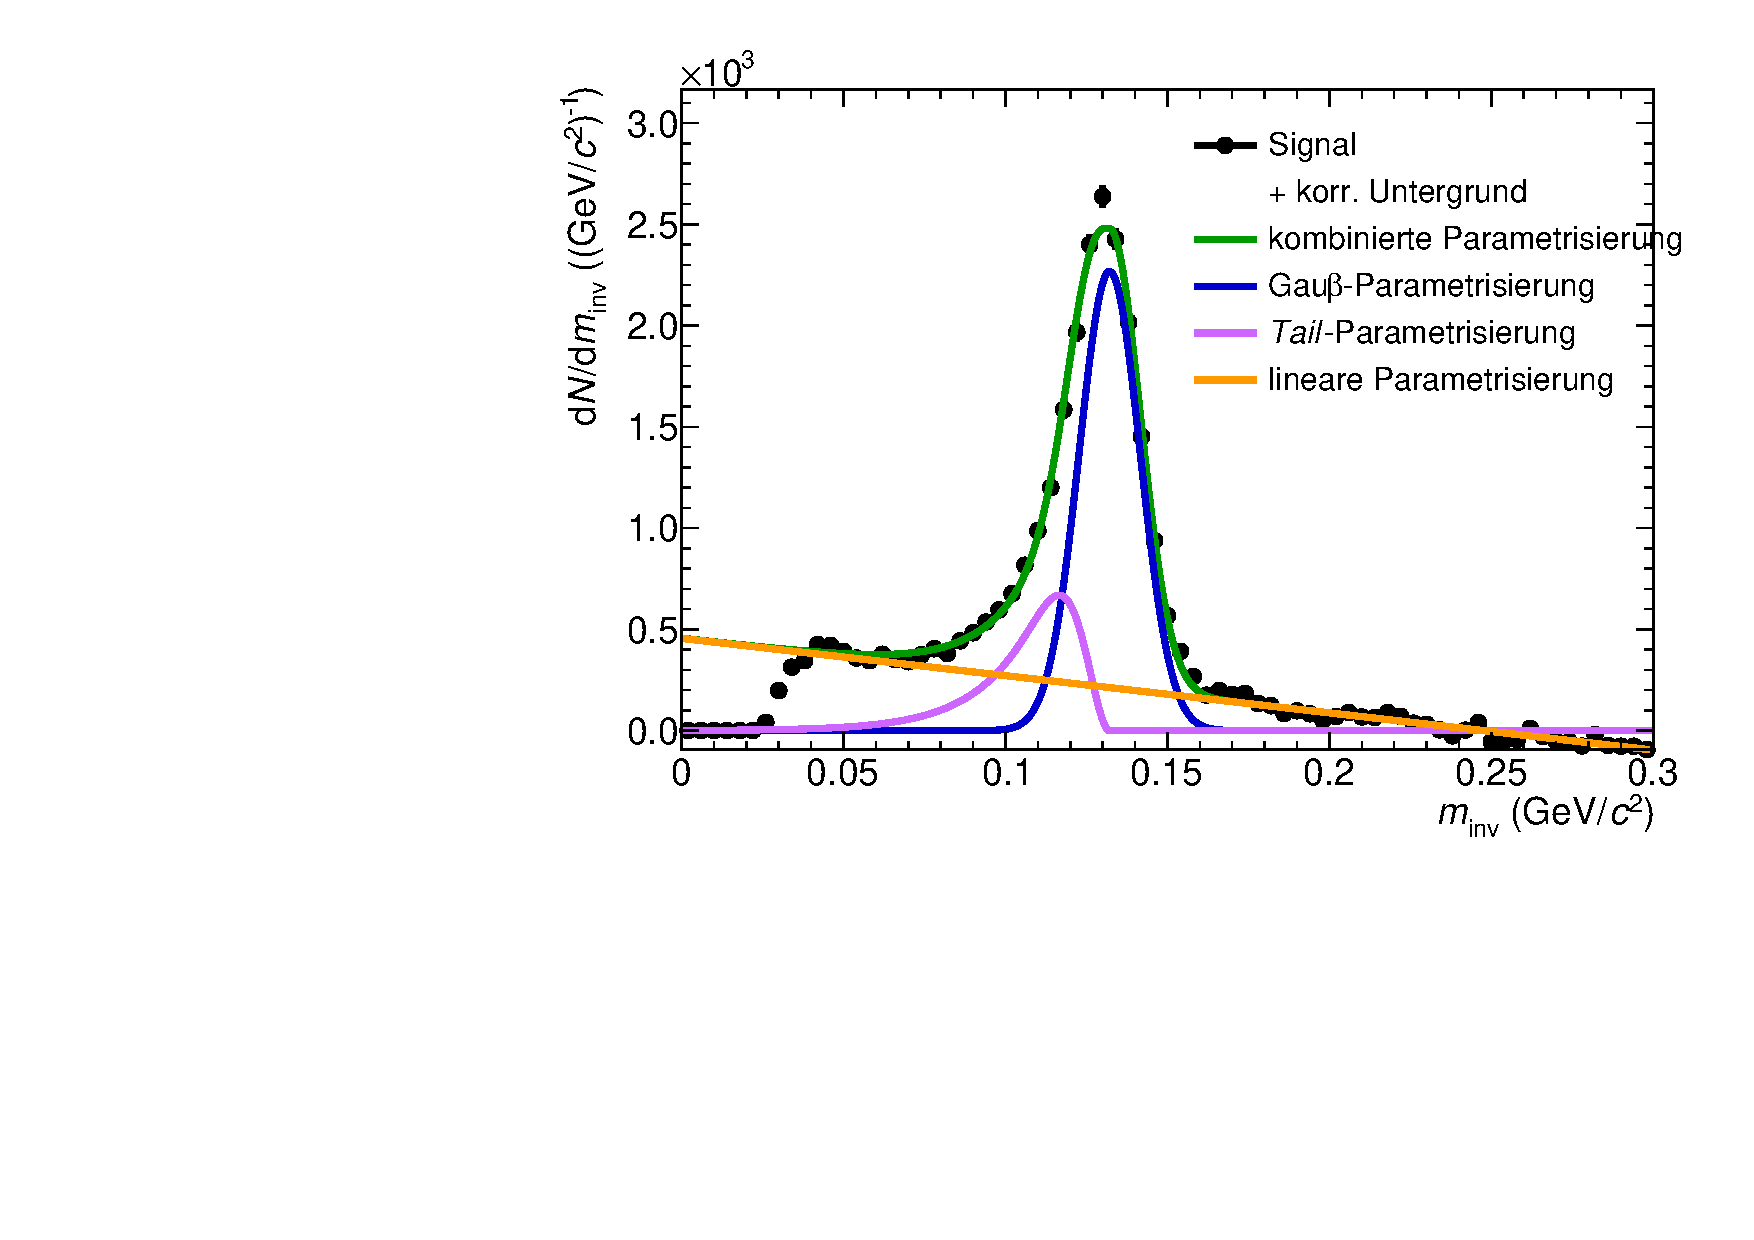
\includegraphics[width=.75\linewidth]{StandardParam.pdf}
\caption{Signal mit korreliertem Untergrund sowie den Funktionen zur Beschreibung des Signals mit korreliertem Untergrund.}
\label{figStandardParam}
\end{figure}
\newline
Abbildung \ref{figStandardParam} zeigt die Verteilung der invariante Masse bestehend aus Signal und korreliertem Untergrund, sowie das Ergebnis einer beschriebenen Anpassung.
Die grüne Kurve entspricht der Summe der drei einzelnen Komponenten, wobei die Gauß-Funktion in blau, die \textit{Tail}-Funktion in pink und die lineare Funktion in orange, dargestellt werden.
Dabei wird deutlich, dass durch die Abschätzung des korrelierten Untergrunds über die lineare Funktion bei einer invarianten Masse von etwa $0\,06\text{ GeV}/c^{2}$, kein beziehungsweise kaum Signal vorliegt.
Zu noch kleineren Massen hin schneidet die Anforderung an den Öffnungswinkel in den Verlauf, welcher nicht durch die Funktionen beschrieben wird.
\newline
Im folgenden Abschnitt wird die Abschätzung des korrelierten Untergrunds mit Hilfe von Templates beschrieben.